% =============================================================================
% s7_c3_boundary.tex --- §7 C3 honest-boundary section (NEW draft, W4 reorder).
%
% SERVES: Claim C3 (honest boundary --- enhancement is not a panacea ->
%         the query-for-retake gate's hardest motivation).
% LEVERS: C3.2 (E5 per-class melanoma net-negative salvage) + C3.3 (v6 mask-L1
%         null) -> §7.4;  C3.1 (E6 severe boundary) + retake routing -> §7.8.
%
% SOURCE/MIGRATION: main.tex §7.3 salvage L402-461 (E5 per-class + E6 severe +
%   Thm2 P1/P3 routing) ; E5 v6 mask-L1 text reused from
%   drafts/s74_branches.tex Branch B ("mask-L1 does NOT help melanoma" verdict,
%   v6 melanoma salvage 5.2% -> 5.2% null, net -81 -> -79).
%
% LOCKED NUMBERS (STORY_FRAMEWORK.md locked table, verifier-checked --- DO NOT
%   invent / DO NOT alter):
%   E5  aggregate moderate salvage 0.737 (benign-dominated; NOT a pass metric);
%       per-class benign 75.6% (1809/2392), benign damage 0.6% (50/8138),
%       melanoma salvage 5.2% (4/77), melanoma damage 31.0% (85/274),
%       net -81 malignant cases; n=3627 per severity; run_id 1441301-batch
%       (results/e5_salvage_persample.csv).
%   E5 v6 mask-L1: melanoma salvage 5.2% -> 5.2% null (4/77), damage 30.3%
%       (83/274), net -81 -> -79 (noise); lambda_mask=3.0, 4x lesion weight;
%       job 1442696/1444753 (results/e5_salvage_v6_persample.csv).
%   E6 severe: dAUC -0.0559 CI[-0.085,-0.028] excluding 0, dflip 0.46;
%       run_id 1441321 (results/e6_severe.csv).
%   Retake routing (Thm2 P1/P3): retake fraction 0.055 [0.031,0.083] high band,
%       0.651 [0.600,0.705] moderate, 0.889 [0.800,0.978] severe (migrated from
%       main.tex L436-461; re-verify with verifier before merge -> \todo).
%
% RED LINES OBSERVED:
%   - aggregate 0.737 used ONLY as a "not-a-pass" counter-example, never claimed
%     as a capability (C3.2 red line).
%   - retake routing phrased as a LOCAL trigger / per-band statement only;
%     NEVER "agent global risk <= Direct" / "triage globally better than direct
%     diagnosis" (STORY R11 / drift def. #3).
% =============================================================================

\subsection{The Honest Boundary: When Enhancement Hurts Diagnosis}\label{sec:exp-boundary}

% --- §7.4 E5 honest salvage (benign-dominated + melanoma net-negative + v6 null) -----

\paragraph{E5 --- salvage rate is benign-dominated, and mask-weighted reconstruction does not
close the gap.}
On the moderate band the aggregate salvage rate --- the fraction of degraded-then-misclassified
images that enhancement restores to a correct prediction --- is $0.737$. This number nominally
clears any modest efficiency target, but it is misleading on its own and we deliberately do
\emph{not} report it as a headline capability: a per-class split (independent EfficientNet-B3
probe, $n=3627$ per severity) shows it is almost entirely benign false-positive correction. The
salvage and damage denominators are distinct subsets: salvage is taken over the
degraded-then-misclassified images, while damage is taken over those the probe originally
classified correctly. On benign lesions, enhancement salvages $75.6\%$ ($1809/2392$
misclassified) while damaging only $0.6\%$ ($50/8138$ correctly-classified); on melanoma it
salvages just $5.2\%$ ($4/77$ misclassified) while damaging $31.0\%$ ($85/274$
correctly-classified) --- a \emph{net loss of $81$ malignant cases}. Enhancement therefore helps
the benign-leaning errors that least need help and harms the malignant cases that matter most,
mirroring the residual dangerous flips reported above (\cref{fig:dflip}) and the severe-band
degradation below. We read the aggregate $0.737$ not as a salvage benchmark to maximise but as a
cautionary example of how an aggregate can hide a class-conditional safety failure.

\paragraph{Mask-weighted reconstruction does not close the malignant gap (v6, honest null).}
We tested whether the malignant-salvage deficit is an artefact of the reconstruction loss ---
specifically, whether the enhancer simply smooths over the lesion. We retrained with a
\emph{mask-weighted} reconstruction objective ($\lambda_{\text{mask}}=3.0$, applying a $4\times$
weight to the lesion region so the enhancer cannot smooth over the lesion itself). The result is a
null (\cref{fig:e5-salvage}): melanoma salvage stays at $5.2\%$ ($4/77$, unchanged from the feature-DP
model) while damage moves only marginally to $30.3\%$ ($83/274$), for a net of $-79$ malignant cases ---
statistically
indistinguishable from the feature-DP result's $-81$. Reweighting the reconstruction loss toward
the lesion is therefore \emph{not sufficient} to close the malignant salvage gap. The failure mode
is not ``the enhancer smooths away the lesion'' but something the per-pixel reconstruction
objective cannot reach: the diagnostic decision boundary depends on texture statistics that
mask-weighted $L_1$ does not target. We report this negative result rather than omit it. We read
E5 --- the benign-dominated aggregate, the net-negative melanoma rescue, and the v6 null together
--- as the strongest evidence that \emph{blanket} enhancement is unsafe and that a query-for-retake
gate is required. This is a genuine safety mechanism, not a project shortcoming: the gate exists
precisely because reconstruction-loss surgery cannot recover the malignant cases. Closing the
malignant salvage gap by other means (e.g.\ diagnosis-aware or adversarial objectives) is left to
future work (\cref{sec:discussion}).

\begin{figure}[t]
  \centering
  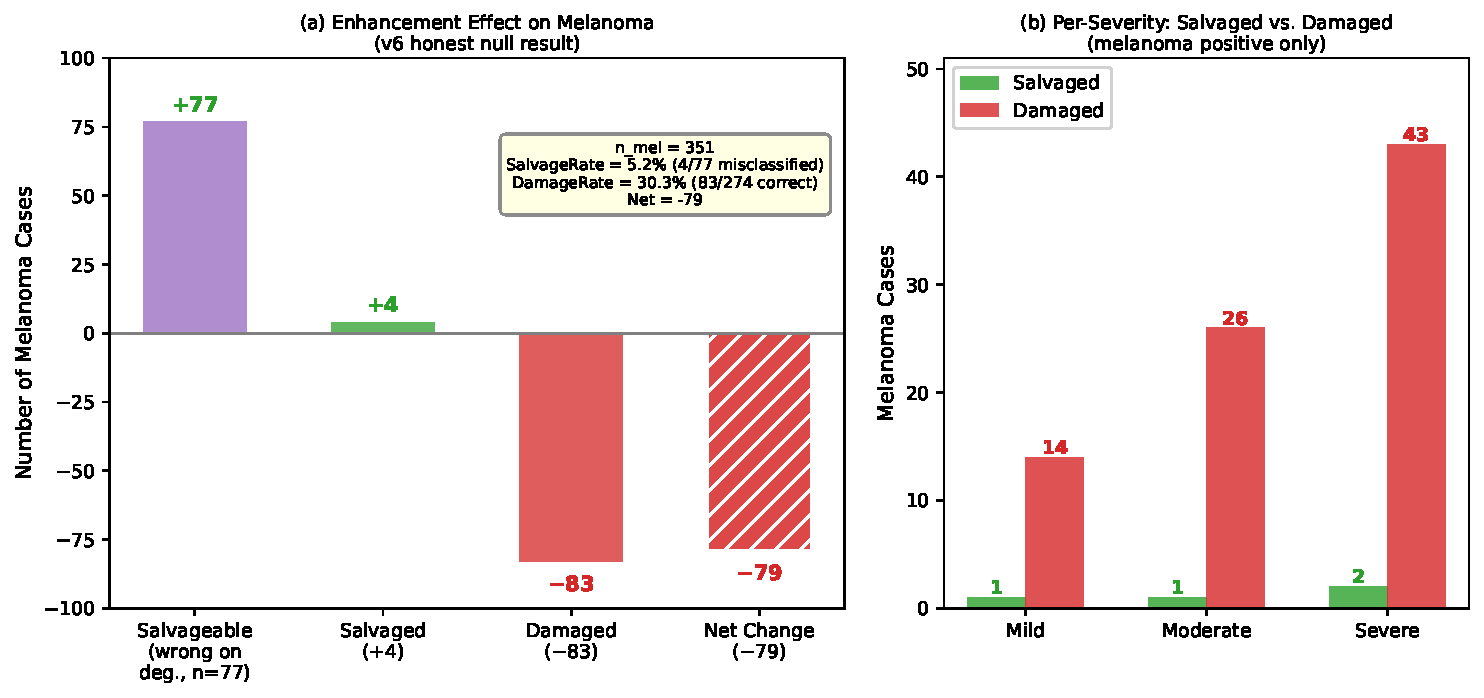
\includegraphics[width=0.92\linewidth]{../../report/figures/fig_e5_salvage_v6.pdf}
  \caption{\textbf{Enhancement is net-negative on melanoma (E5, mask-weighted v6 honest null).}
  \textbf{(a)} Of the $77$ melanomas misclassified after degradation, enhancement salvages only
  $4$ ($5.2\%$), while damaging $83$ of the $274$ originally-correct melanomas ($30.3\%$), for a
  net change of $-79$ malignant cases. \textbf{(b)} The deficit holds at every severity (salvaged
  versus damaged: $1/14$ mild, $1/26$ moderate, $2/43$ severe). Source
  \texttt{results/e5\_salvage\_v6\_persample.csv}. The mask-weighted reconstruction objective
  ($\lambda_{\text{mask}}=3.0$, $4\times$ lesion weight) leaves the malignant salvage rate
  unchanged, confirming the gap is not a smoothing artefact.}
  \label{fig:e5-salvage}
\end{figure}

% --- §7.8 E6 severe boundary + retake routing (migrated from main.tex L429-461) ------

\paragraph{E6 --- the severe-degradation safety boundary.}
On the severe band we observe the boundary directly: enhancing severely degraded images
significantly \emph{lowers} diagnostic AUC ($\Delta\mathrm{AUC}=-0.0559$, $95\%$ CI
$[-0.085,-0.028]$, excluding zero) and induces a $0.46$ dangerous-flip rate (run\_id 1441321).
Enhancement is the wrong action in this regime; the agent routes severe inputs to query-for-retake
rather than enhance-then-diagnose (\cref{sec:agent}), which is exactly the safety behaviour the
salvage boundary is meant to enforce.

\paragraph{Why these results, taken together, motivate routing to retake rather than enhancement.}
The decision to route a degraded input to query-for-retake rather than to enhance-then-diagnose is
not driven by a single aggregate quality reading; it rests on three distinct, empirically grounded
triggers, each at a different granularity. First, the \emph{per-class} melanoma evidence: on
melanoma, enhancement salvages only $5.2\%$ while damaging $31.0\%$, a net loss of $81$ malignant
cases (E5, above), so the cases that matter most are precisely those enhancement cannot rescue.
Second, the \emph{mixed-severity} boundary: on the severe band enhancement significantly lowers
diagnostic AUC ($-0.0559$, CI excluding zero; E6, above). Third, the \emph{per-dimension} extreme:
on the most degraded contrast setting, the decision-surface analysis finds enhancement to
significantly hurt recoverability (\cref{sec:exp-surface}), one per-dimension trigger that
complements --- and does not replace --- the per-class and mixed-severity evidence. That these
triggers live at different granularities is exactly the point: the reliability axis of the
decision surface already shows that a triage policy treating degradation as a \emph{single scalar}
would mis-prioritise the dimensions that actually erode diagnosis (\cref{sec:reliability-axis}), so
the retake decision must be conditioned jointly on per-class risk, severity, and the specific
degradation dimension rather than on one summary number.

\paragraph{The retake channel fires monotonically with degradation (Theorem~\ref{thm:agent-compact}
P1/P3).}
The complement of the salvage boundary is the retake channel, and its empirical behaviour matches
the threshold-window structure of Theorem~\ref{thm:agent-compact}. As quality drops, the fraction
of cases the agent routes to query-for-retake increases strictly and monotonically across the
three quality bands (\cref{fig:retake-gradient}): $0.055$ on the high band ($95\%$ CI $[0.031,0.083]$),
$0.651$ on the moderate band ($[0.600,0.705]$), and $0.889$ on the severe band ($[0.800,0.978]$;
bootstrap CIs, all non-overlapping).% \todo{verifier: re-check retake-fraction CIs migrated from main.tex L441-442 against results source before merge}
This is the realised counterpart of the policy: the retake action is essentially dormant where
direct diagnosis suffices (P3) and dominates exactly where enhancement is unsafe (P1), so the
channel that the severe-band boundary above calls for is precisely the channel the policy
activates. We emphasise that this is a statement about \emph{routing}, not about enhancement
efficacy: the aggregate salvage rate on the severe band ($0.898$) is benign-dominated in the same
way as the moderate band quantified above, and is \textbf{not} evidence that enhancement helps
severe malignant cases --- the correct action on the severe band is to route to retake ($0.889$),
not to enhance, which is exactly what Theorem~\ref{thm:agent-compact} P3 prescribes.

\begin{figure}[t]
  \centering
  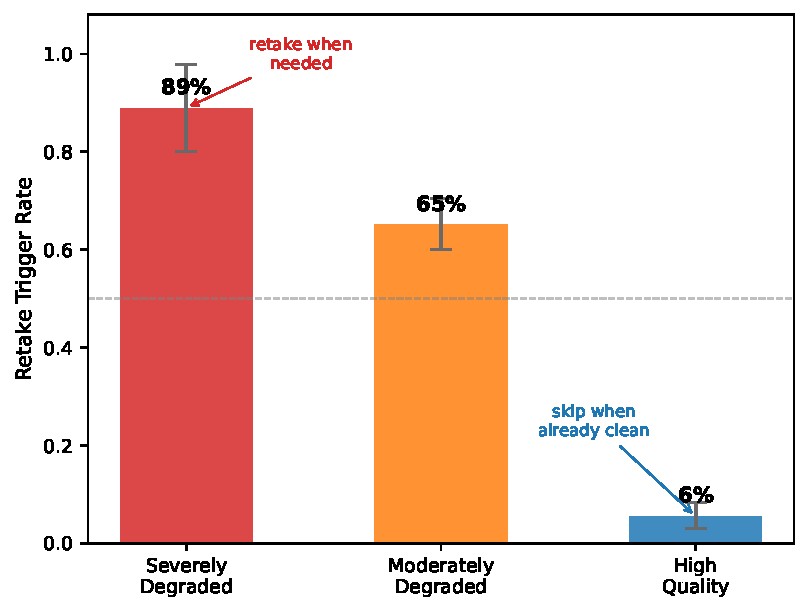
\includegraphics[width=0.58\linewidth]{../../report/figures/fig_retake_gradient.pdf}
  \caption{\textbf{The query-for-retake channel fires monotonically with degradation.}
  Fraction of cases the agent routes to query-for-retake across the three quality bands,
  with bootstrap $95\%$ confidence intervals (source
  \texttt{results/agent\_vs\_direct\_risk.csv}): $0.055$ (high), $0.651$ (moderate),
  $0.889$ (severe); the intervals are mutually non-overlapping. The channel is essentially
  dormant where direct diagnosis suffices and dominates exactly where enhancement is unsafe,
  realising the threshold-window policy of Theorem~\ref{thm:agent-compact}.}
  \label{fig:retake-gradient}
\end{figure}

\paragraph{Local, per-band reading only.}
Where the policy does route an input to the enhance channel, the same per-quality routing yields
risk reductions relative to direct diagnosis whose CIs exclude zero \emph{within each band}
(severe $-0.305$, CI $[-0.390,-0.214]$; moderate $-0.189$, $[-0.204,-0.174]$; high $-0.127$,
$[-0.136,-0.119]$),% \todo{verifier: re-check per-band risk-reduction CIs migrated from main.tex L451-453}
and the moderate-band enhancement salvage of $0.778$ on the narrower routed sub-band clears a
modest efficiency target. This $0.778$ is measured on a different, narrower population than the
$0.737$ aggregate above: it is computed only on the cases the policy actually routes to the enhance
channel (the moderate quality sub-band $\bar{q}\in[0.35,0.5]$, $n=3253$), whereas the $0.737$ is
taken over the full moderate-severity split ($n=3627$). It is therefore subject to exactly the same
benign-dominated caveat as the rest of this section: it reflects predominantly benign
false-positive correction on a benign-prevalent cohort, and is \textbf{not} evidence that
enhancement improves diagnosis of severe or malignant lesions. We stress that these are
\emph{local, per-band} statements about where routing applies the enhance action conditionally;
they do \textbf{not} claim that the agent's global risk is at most that of direct diagnosis, nor
that quality-aware triage globally outperforms direct diagnosis. The honest global comparison ---
where fixed-threshold triage is \emph{not} found to outperform direct diagnosis --- is reported
separately (\cref{sec:exp-triage}). With that caveat, the gains the bound predicts on the salvage
band are realised locally while the unsafe severe cases are diverted to retake rather than
enhanced.
